\documentclass[12pt]{article}
\usepackage{graphicx}
\usepackage{amsmath}
\usepackage{fullpage}
\usepackage{amssymb}
\usepackage{amsfonts}
\usepackage{latexsym}
%\usepackage{pstricks}
\usepackage{tikz,pgflibraryplotmarks}
\usepackage{algorithm}
\usepackage{algpseudocode}
\usepackage{hyperref}
\usepackage[nottoc,numbib]{tocbibind} 

\newcommand {\R}    {{\rm I\!R}}
\newcommand {\bu}   { {\bf u} }   	% discrete flow field
\newcommand {\buref}   { {\bf u}_{\text{ref}} } % discrete reference flow field
\newcommand {\bugt}   { {\bf u}_{\text{gt}} } 	% discrete ground truth flow field
\newcommand {\bfx}  { {\bf x} }
\newcommand {\bfc}  { {\bf c} }
\newcommand {\bfd}   { {\bf d} }
\newcommand {\bfv}   { {\bf v} }
\newcommand {\bfe}   { {\bf e} }
\newcommand {\bfw}   { {\bf w} }
\newcommand {\bfs}   { {\bf s} }
\newcommand {\bsgt}   { {\bf s_\text{gt}} }
\newcommand {\bfu}   { {\bf u} }
\newcommand {\bfq}   { {\bf q} }
\newcommand {\bfp}   { {\bf p} }
\newcommand {\bfz}   { {\bf z} }
\newcommand {\bfy}   { {\bf y} }
\newcommand {\bfk}   { {\bf k} }
\newcommand {\bfm}   { {\bf m} }

\newcommand {\bfK}  { {\bf K} }
\newcommand {\bfP}  { {\bf P} }
\newcommand {\bfA}  { {\bf A} }
\newcommand {\bfB}  { {\bf B} }
\newcommand {\bfG}  { {\bf G} }
\newcommand {\bfF}  { {\bf F} }
\newcommand {\bfI}  { {\bf I} }
\newcommand {\vu}  { {\vec {\bf  u}} }   % continuous flow field
\newcommand {\vuref} {\vu_{\text{ref}}}  % continuous reference flow field
\newcommand {\vq}  { {\vec {\bf  q}} }
\newcommand {\ve}  { {\vec {\bf  e}} }
\newcommand {\vh}  { {\vec {\bf  h}} }
\newcommand {\vx}    {\vec {\bf x}}     
\newcommand {\bx}    {{\bf{x}}}     
\newcommand {\bfr}    {{\bf{r}}}     
\newcommand {\bflambda}    {{\boldsymbol{\lambda}}}     
\newcommand {\blambda}	 { {\boldsymbol \lambda} }
\newcommand {\bmu}    	 { {\boldsymbol \mu} }
\newcommand {\zero}   	 { {\bf 0} }
\newcommand {\gb}      	 { {\bf g} }
\newcommand {\bnabla}	 { { \boldsymbol \nabla} }
\newcommand {\btheta}	 { { \boldsymbol \theta} }
\newcommand {\balpha}	 { { \boldsymbol \alpha} }
\newcommand {\bfxi}		 { { \boldsymbol \xi} }
\newcommand{\hf}		 {\frac12}
\newcommand{\hx}[1]		{{\ensuremath{h^x_{\scriptscriptstyle #1}}}}
\newcommand{\hy}[1]		{{\ensuremath{h^y_{\scriptscriptstyle #1}}}}
\newcommand{\hz}[1]		{{\ensuremath{h^z_{\scriptscriptstyle #1}}}}
\newcommand{\E}			{\vec{E}}
\newcommand{\A}			{\vec{A}}
\renewcommand{\H}		{\vec{H}}
\newcommand{\J}			{\vec{J}}
\newcommand{\F}			{\vec{F}}
\newcommand{\M}			{\vec{M}}
\newcommand{\s}{\vec{s}}
\newcommand{\h}{\vec{h}}
\newcommand{\sig}{\sigma}
\newcommand{\nn}{\vec{n}}
\renewcommand{\div}{\nabla\cdot\,}
\newcommand{\grad}{\ensuremath {{\bf{ \nabla}}}}
\newcommand{\curl}{\ensuremath{{\nabla}\times\,}}
\newcommand{\alert}[1] {\textcolor{red}{#1}}
\newdimen\iwidth\iwidth=30mm
	\newcommand{\rottext}[1]{\rotatebox{90}{\hbox to 30mm{\hss #1\hss}}}
\newcommand{\rme}{\rm{e}}
\newcommand{\HRule}{\rule{\linewidth}{0.25mm}}
\newcommand{\bA}  { {\bf A} }      % transport matrix
\newcommand{\bB}  { {\bf B} }      % matrix for initial condition of hyperbolic problem, B=[T;0;...;0]
\newcommand{\bc}  { {\bf c} }      % time series of concentration, c = [c1,...,cN]
\newcommand{\bI}  { {\bf I} }      % identity matrix
\newcommand{\bF}  { {\bf F} }      % tomography matrix
\newcommand{\bG}  { {\bf G} }      % image gradient, G = dT = GRAD( T * s)

\newcommand{\bK}  {\text{{\bf K}}} % design Geophysics matrix
\newcommand{\bT}  {\text{\bf T}} % push forward matrix
\newcommand{\bM}  {\text{{\bf M}}} % interpolation matrix
\newcommand{\bfJ}  {\text{{\bf J}}} % interpolation matrix
\newcommand{\bfW}  {\text{{\bf W}}} % design weights matrix
\newcommand{\bfL}  {\text{{\bf L}}} % regulariztion operator matrix
\newcommand{\bfE}  {\text{{\bf E}}} % regulariztion operator matrix
\newcommand{\JJ}  {\mathcal{J}}    % objective functional
\newcommand{\cD}  {\mathcal{D}}    % data misfit
\newcommand{\CR}  {\mathcal{R}}    % regularization functional
\newcommand{\CRflow}  {\mathcal{R}^{\text{flow}}}    %  flow 
\newcommand{\CRsat}   {\mathcal{R}^{\text{s}}}     %  saturation 
\newcommand{\CF}  {\mathcal{F}}    % continuous tomography operator
\newcommand{\sh}  {\texttt{s}}     % discretized initial slowness
\newcommand{\DIVh}   {{\textsf{DIV}}}  % discretized divergence 
\newcommand{\CURLh}  {{\textsf{CURL}}} % discrete curl operator
\newcommand{\GRADh}  {{\textsf{GRAD}}} % discrete gradient operator
\newcommand{\W}{\text{\bf W}}
\newcommand{\C}{\text{\bf C}}
\newcommand{\shat}{\widehat{s_0}}
\newcommand{\shatk}{\widehat{s}}
\newcommand{\mhat}{\widehat{\bf m}}
\newcommand{\what}{\widehat{\bf w}}
\newcommand{\Sig}{\bf \Sigma_m }
\newcommand{\Sigh}{\bf \Sigma}

\def\kronecker{\raisebox{1pt}{\ensuremath{\:\otimes\:}}} 
\sloppy



\begin{document}

\title{Optimal experimental design for reservoir monitoring}
\author{J. Fohring and E. Haber }


\maketitle
\begin{abstract}
Efficiently monitoring subsurface flow using geophysical imaging techniques is important to several applications such as aquifer characterization or enhanced oil recovery projects.
To increase efficiency, the optimal number of measurements and their locations required for a geophysical survey are computed by an A-optimal experimental design method for ill -posed problems. 
A-optimal design minimizes the prior covariance matrix associated with target subsurface model. To obtain a prior covariance matrix for the future unknown model, the posterior covariance matrix associated with the current MAP model estimate is propagated forward in time. The MAP estimate is computed from historic geophysical data. The method is demonstrated for a two dimensional borehole seismic tomography experiment and a three dimensional DC resisitivity survey. An advection model  was applied to describe subsurface flow and  propagate the error covariance matricies forward in time. 
 


\end{abstract}



\section{Introduction} 
\begin{itemize}

\item Monitoring; May problems in geophysics address the issue of monitoring subsurface flow, such as aquifer characterization, enhanced oil recovery, or saltwater intrusion. In general one would like to image the motion of certain subsurface parameters over a period of time.  One method to do so is to collect measurements dependent on these parameters and invert through a mathematical relationship to recover parameter distributions. When monitoring for these dynamic parameters, the choice of where the data are collected becomes important as resolution is both temporally and spatially dependent. 

\item much has been done in experimental designs for linear and nonlinear problems...A optimal, etc.. appropriate references. inverting for fluid parameters given geophysical imaging...refs...talk about seismic, and helmolz and simultaneous sources

\item Determining an the design of the data collection experiment requires knowledge of the target parameter distribution. Typically optimal experimental design methods rely on minimizing the posterior error associated with inverting and thus imaging the parameter distribution. This poses a problem, particularly for static cases, since the point of  the data collection is to image the unknown target. However, if the dynamics governing the motion of the unknown target are known, even to a small degree in accuracy, then it is possible to design the data collection experiment to be conducted in the future as the target moves. In order to design for a future experiment it is necessary to know the initial distribution of target parameters as well as the dynamics. If the initial condition is provided with the dynamics, then either an iterative approach or and all at once approach can be taken to determine date collection designs for a set of time points. 

\item An all at once method would seek to recover all of the designs for a set of time points given the dynamics and the initial condition. This method requires and 'all at once' prior covariance matrix. The generation of such a matrix is difficult... This method also puts a great deal of trust into the dynamic model. If for example, the velocity field in which a tracer is advected is known to very low accuracy then the designs and location of the tracer target far into the future would have significant error. 
\item An iterative or adaptive design method would make use of data collected for each experiment to update both the current covariance matrix and can be used to update the dynamic model parameters as well. This way, after each data collection experiment is conducted a design for the next time is computed with higher accuracy information.
\item computational limitations: covariance matrices are large and dense, not necessarily spd, making factorization/ reduction techniques difficult. geophysical experiments are computationally expensive. Helmholz- simutaneous source...

\end{itemize}




\section{A-Optimal experimental design for linear ill-posed problems} 
To begin, a brief review of A-optimal experimental design for ill-posed problems is given as presented in full detail in \cite{habera}. 

\bigskip

Consider the discrete static ill-posed inverse problem of estimating  model parameters $\bfm \in \mathbb{R}^{N}$ from noisy observation data $\bfd \in \mathbb{R}^{M}$,
\begin{equation*}
\bfd - \bfF \bfm = {\bf \epsilon},
\end{equation*} 
where $\bfF$ is an $M \times N$ matrix with each row representing an experiment. 
 
Assuming a Bayesian approach is taken with the posterior estimate  $\mhat$ conditioned on a known prior distribution $\pi_m = N({\bf \mu},\Sig)$, and that the error ${\bf \epsilon}$, is Gaussian $N(0,\W^{-1})$, the Bayesian posterior estimate is obtained by minimizing the negative log-likelihood of Bayes rule,
\begin{eqnarray*}
\mhat(\bfw) &=& \text{ argmin } (\bfF \bfm- \bfd)^{\top} \W(\bfF \bfm- \bfd) + (\bfm-{\bf \mu})^{\top}\Sig^{-1}(\bfm-{\bf \mu})\\
 &=& (\bfF^{\top} \W \bfF + \Sig^{-1})^{-1}(\bfF^{\top} \W \bfd_w + \Sig^{-1}{\bf \mu}).
\end{eqnarray*}     
 The weighting matrix $\W = \text{diag}[\bfw] \text{ and } \bfw = (\omega_1,..,\omega_M)^{\top}$, relates to the data variance as Var($d_{i}$) $=1/\omega_i$. 
\bigskip

%    A-optimal experimental designs for ill-posed problems  take the same Bayesian approach, where the posterior estimate  $\mhat$ is conditioned on a known prior distribution for $\bfm$. A design is chosen which minimizes the average mean squared error under the prior, that is,  the Bayes risk \cite{Habera}.  
   
   

  A-optimal experimental designs for well-posed inverse problems are defined by  minimizing the average variance of the estimate $\mhat$, with covariance matrix $\Sig$ \cite{Atkinson1992}. To this end, minimizing the average variance is equivalent to minimizing the trace of the posterior covariance matrix,
  % Therefore, the Bayes risk of the Bayesian estimator $\mhat$ is given by
  \begin{equation}
  \label{AB}
  \phi_{A_B}(\bfw) = \text{tr}[(\bfF^{\top} \W \bfF + \Sig^{-1})^{-1}].
  \end{equation}


Given $\phi_{A_B}$, a design can be computed by solving a sparsity controlled optimal design optimization problem \cite{Haber2008}. The design weights $\omega_i$ are determined  by minimizing  $\phi(\bfw)$ with an $\l_1$ penalty on  $\bfw$ to promote sparsity,
\begin{subequations}
\label{design}
\begin{eqnarray}
&\widehat{\bfw}& = \text{ arg min } \phi(\bfw) + \beta\|\bfw\|_1\\
 &\text{ s.t.}& 0 \geq \omega_i.
\end{eqnarray}
\end{subequations}
It is important to note that in this formulation $\mhat$ is chosen to be a linear (or affine) function of the data, although  other estimators could be used, such as a Tikhonov estimator. Since the idea is to  design experiments at future time steps for dynamic problems  where the estimators covariance matrix can be estimated, the simple Bayesian estimator is sufficient.









\subsection{Designing experiments for dynamic model parameters}
\label{dynamicDesign}
To illustrate the method of estimating the covariance matrix associated with a future model, we first consider the dynamic  tracer advection problem \cite{Chen2006}, which describes the transport of a solute in a fully saturated porous media 
\begin{subequations}
\label{floweq}
\begin{eqnarray}
 \label{eq:flow}
&&\frac{\partial( c \rho)}{\partial t} + \div c \rho \vu  = 0,\\
\nonumber
 &&\text{ subject to } c\rho(0,\vx) = c_0\rho(\vx),
\end{eqnarray}
  with hydraulic conductivity $\bfK$, and tracer concentration $c$ in a fluid of density $\rho$. The fluid velocity field $\vu$ satisfies a simple source-sink ($q$) flow model
\begin{eqnarray}
\label{eq:flowp}
&&  \div  \vu =   q \\ % \mu^{-1}\bfK(\bfx) \grad p
\label{eq:flowu}
&& \vu =  \bfK(\vx)  \grad p \\
\label{eq:incond}
&&  p(0,\vx) = p_0(\vx),
\end{eqnarray}
\end{subequations}
 with either Dirichlet or Neumann boundary conditions on the pressure $p$.\\
%

With the goal being to image the motion of the tracer, $c(t,\vx)$, we assume that changes in $c$ amount to changes in geophysical properties. This implies that $m(c)$ exists, and that the motion of $m$ is governed by Equation \eqref{eq:flow}. 


Since Equation \eqref{eq:flow} is linear with respect to $c$, a particle in cell discretization was chosen. Applying this discretization technique on a uniform grid with $c$ at the cell centers and $\vu$ on the edges,  results in the  following linear transformation:
\begin{equation}
\bfm _{k+1} = \bT(\bfu)\bfm_k,
\end{equation}  
where the transport matrix $\bT$ is an interpolation matrix dependent only on the velocity field $\bfu$, see \cite{Fohring2014} for more details. 

\bigskip


%Assuming that either an initial convariance matrix can be estimated for $\mhat_0$, from either an initial data set or error estimate, then designs can be estimated for future surveys. 

Given an imaging data set for time $k$, an estimate $\mhat_k$ can be computed in the usual way such that $\mhat_k$ is a random  variable with  a Gaussian distribution. 
Since the linear transformation of a Gaussian random variable is also a random variable, then  
\begin{eqnarray*}
\mhat _{k+1} &=& \bT(\bfu)\mhat_k,\\
 \Sigh_{k+1} &=& \bT \Sigh_{\mhat_k} {\bT}^{\top},
\end{eqnarray*}  
 (See \cite{Maybeck1979} for a complete proof).
That is, the posterior covariance matrix $\Sigh_{\mhat_k}$ associated with  $\mhat_k$ is propagated forward in time with the known dynamics of the problem. This provides the prior distribution required to compute an A-optimal experimental design for the next survey at the time point $k+1$.

The basic algorithm illustrating the design process for a linear observation method is outlined in Algorithm \ref{Alogrithm}. 
%%%%%%%%%%%%%%%%%%%%%%%%%%%%%%%%%%%%%%%%%%%%%%%%%%%%%%%%%%%%%%%%%%%%%%%%%%%%%%%%%%%%%%%%
\begin{algorithm}
\caption{Iterative Optimal $\phi_{A_{B}}$Design}\label{Alogrithm}
\begin{algorithmic}[1]
%
\State $\text{Initialize: }\Sigh_0$
\Comment{estimate from prior information before going to the field!}
%
\For{$k = 1 \text{ to } n$}  
\Comment{$n$ is the maximum number of experiments, or time points}
%
\State $\what_k(\Sigh_k) \to \text{diag}(\what_k)\bfF = \bfF_k $ \Comment{ compute the optimal design by solving \ref{design}}
%
\State $\bfd_k = \bfF_k \bfm_k + \epsilon_k$
\Comment{collect data}
%
\State $\mhat_k = (\bfF_k^{\top}\bfF_k +\alpha \bfL^{\top} \bfL)^{-1}\bfF_k^{\top} \bfd_k  $
\Comment{estimate the current model}
%
\State $\Sigh_{k} \gets {\bT}(\bfF_k^{\top} \bfF_k +\alpha \bfL^{\top} \bfL)^{-1}\;{\bT}^{\top}$ 
\Comment propagate the error
%
\EndFor\label{euclidendwhile}
%%%%%%%%%%%%%%%%%%%%%%%%%%%%%%%%%%%%%%%%%%%%%%%%%%%%%%%%%%%%%%%%%%%%%%%%%%%%%%%%%%%%%%
\end{algorithmic}
\end{algorithm}
In this algorithm  $\mhat_k$ is estimated using a Tikhonov method with a regularization operator $\bfL$. To design the experiment, only data from the current time step is used, and the velocity field $\bfu$ is given.

\subsection{Numerical optimization for dynamic A-optimal design}
Finding an optimal design for the time step $k+1$ involves solving the optimization problem \ref{design} by minimizing the objective functional,
\begin{equation}
\label{traceObj}
\JJ_{k+1}(\bfw) = \text{tr}[(\bfF^{\top} \text{diag}(\bfw) \bfF + \Sigh_{k+1}^{-1})^{-1}] + \beta \bfe^{\top}\bfw,
\end{equation}
where $\bfe$ is a vector of ones.

This is a difficult task for large problems, particularly due to the trace of a large dense matrix, the computation of the derivative of the trace, and the requirement of the inverse of the large, dense propagated posterior covariance matrix $\Sigh_{k+1} = {\bT}(\bfF_k^{\top} \bfF_k +\alpha \bfL^{\top} \bfL)^{-1}\;{\bT}^{\top}.$ To this end, several actions can be taken to reduce the computational costs.

First, a stochastic Hutchinson trace estimator is used to approximate the trace  \cite{Hutchinson1989,habera} such that Equation \eqref{traceObj} can be written as
\begin{equation}
\label{Obj}
\JJ_{k+1}(\bfw) = \bfv^{\top}(\bfF^{\top} \W \bfF + \Sigh_{k+1}^{-1})^{-1}\bfv + \beta \bfe^{\top}\bfw,
\end{equation}
where $\bfv$ is a random vector with values $1$ and $-1$ with equal distribution. This approximation makes the computation of the derivative of $\JJ$ tractable for large problems. \\

A second issue arises when computing the derivative  of $\JJ$, as this involves computing the derivative of an inverse matrix, 
\begin{equation*}
\nabla_{\bfw} \JJ_{k+1}(\bfw) =\bfv^{\top} \nabla_{\bfw}\Big((\bfF^{\top} \W \bfF + \Sigh_{k+1}^{-1})^{-1}\bfv \Big) + \beta \bfe.
\end{equation*}
To compute  the derivative of $\JJ$ we define  
\begin{eqnarray}
\label{eq:z}
\bfz = (\bfF^{\top} \W \bfF + \Sigh_{k+1}^{-1})^{-1}\bfv \quad \Leftrightarrow \quad
(\bfF^{\top} \W \bfF + \Sigh_{k+1}^{-1})\bfz = \bfv,
\end{eqnarray}
and differentiate implicitly to obtain 
\begin{eqnarray*}
\bfF^{\top}\text{diag}(\bfF \bfz) + (\bfF^{\top} \W \bfF + \Sigh_{k+1}^{-1})\nabla_{\bfw}\bfz = 0.
\end{eqnarray*}
The gradient of $\bfz$ is then given by
\begin{equation*}
\nabla_{\bfw}\bfz = -(\bfF^{\top} \W \bfF + \Sigh_{k+1}^{-1})^{-1} \bfF^{\top}\text{diag}(\bfF \bfz).
\end{equation*}
\\
Thus, the first term in $\nabla_{\bfw} \JJ_{k+1}(\bfw)$ is
\begin{equation*}
-\bfv^{\top}(\bfF^{\top} \W \bfF + \Sigh_{k+1}^{-1})^{-1} \bfF^{\top}\text{diag}(\bfF \bfz). 
\end{equation*}
Taking the transpose 
\begin{equation*}
-\text{diag}(\bfF \bfz)\bfF(\bfF^{\top} \W \bfF + \Sigh_{k+1}^{-1})^{-1} \bfv
\quad \Leftrightarrow\quad -\text{diag}(\bfF \bfz)(\bfF \bfz) = -\bfF \bfz \odot \bfF \bfz,
\end{equation*}
so that the derivative of the objective function is then 
\begin{equation}
\nabla_{\bfw} \JJ_{k+1}(\bfw) =  -\bfF \bfz \odot \bfF \bfz + \beta \bfe.
\end{equation}
Since the design problem \eqref{design} is nonlinear with respect to $\bfw$, a Newton type iterative method is used with a backtracking line search. This solution method requires both the evaluation of $\JJ$ and  its gradient, which are conveniently obtained by solving for $\bfz$ only once. 

At this point it is important to note that computing $\bfz$ requires the explicit inverse of the prior covariance matrix $\Sigh_{k+1}$. For small scale problems it is possible to compute and store the inverse of this matrix and to use direct solvers to compute $\bfz$. However, there is no guarantee that $\Sigh_{k+1}$ will be positive definite, nor in our case  invertable. 

For case where $\Sigh_{k+1}$ is SPD, Lanczos bidiagonalization can be applied by first reducing the system \eqref{eq:z} to standard form. This process also requires  forming $\Sigh_{k+1}$ and computing its Cholesky factorization. However, the Cholesky factorization is evaluated outside of the design optimization, so depending on the problem size, it is somewhat computationally cheap. 

For large scale problems forming $\Sigh_{k+1}$, computing its inverse explicitly, and storing the resulting large dense matrix becomes intractable. To avoid forming and computing such an expensive matrix, Krylov subspace methods can be applied, such as the Conjugate Gradient method. This allows us to take advantage of matrix vector products and avoid forming $\Sigh_{k+1}$. If, as above, a Tikhonov estimate is used to estimate $\mhat_k$ and thus $\Sigh_k$, then 
\begin{equation}
\Sigh_{k+1}^{-1} = {\bT}^{-\top}(\bfF_k^{\top} \bfF_k +\alpha \bfL^{\top} \bfL)\;{\bT}^{-1}.
\end{equation}
In this way, solving for $\bfz$ with an iterative method requires the solution to the systems:
\begin{eqnarray}
&&\bT(\bfu) \bfy = \bfz\\
&&\bT(\bfu)^{\top} \bfx = (\bfF_k^{\top} \bfF_k +\alpha \bfL^{\top} \bfL)\bfy.
\end{eqnarray}
Given that $\bT$ is sparse, and provided it is non-singular, then $\bfz$ can be computed fairly efficiently without ever forming the posterior covariance at time $k$ or its inverse, and thus never forming or storing $\Sigh_{k+1}^{-1}$. 




\subsection{Understanding the covariance matrix}
It is important to note  that there is no guarantee that $\Sigh_{k+1}$ will be positive definite. In fact it is possible that the transport matrix $\bT$ can  be singular. This generally occurs for zero flux boundary conditions; the assumption being that there is no tracer coming in from outside of the domain.  

The zeros in the transport matrix translate to entries in $\Sigh_{k+1}$ with zero variances, or infinite certainty that there is no mass entering a cell from outside the domain. 
One way to rectify the singularity is to remove this information from the covariance matrix. 

By introducing the $l\times N$ projection matrix $\bfP$, which maps from  $\mathbb{R}^{N}$ to the reduced space $\mathbb{R}^{l}$,  the reduced model and reduced covariance matrix are given by
\begin{eqnarray}
&&\mhat^{\text{r}}_{k+1} =\bfP \bT \mhat_{k},\\
&&\Sigh^{\text{r}}_{k+1} = \bfP \Sigh_{k+1}\bfP^{\top}.
\end{eqnarray}
This is a reasonable approach since the experiment we are designing for depends on where the tracer is currently. Therefore, the cells associated with zero variances will not contribute to the optimal design. This method not only alleviates the singularities, but also reduces the overall size of the problem.  
\alert{SHOW this here, what T looks like, what Sigma looks like}

\bigskip
A second approach requires the inclusion of boundary conditions. In particular, we redefine the estimated model at time $k+1$, 
\begin{equation}
\mhat_{k+1} = \bT \mhat_{k} + \xi_k,
\end{equation}
so that it is composed of the transported estimate plus a random model error which lives just outside the domain. See figure \alert{need a figure to illustrate this}.

In the following section, a simple example is presented to illustrate the different solution methods for a small problem with a given velocity field and small displacement so that $\bT$ is positive definite. 


%%%%%%%%%%%%%%%%%%%%%%%%%%%%%%%%%%%%%%%%%%%%%%%%%%%%%%%%%%%%%%%%%%%%%%%%%%%%%%%%%%%%%%%%%%%%%%%%%%%%%%%%%%%%%%%%%%%%%%%%%%%%%%%%%%%%%%%%%%%%%%%%%%%%% EXAMPLE 1
\section{Numerical example 1: Iterative design, known flow model} % (fold)
To demonstrate  iterative optimal experimental design, two geophysical imaging techniques are considered. First, a travel time seismic tomography geophysical survey is applied to image the advection of a tracer in the subsurface. An initial spatial distribution of the tracer is provided, and the tracer is advected with the flow of water injected from one well and pumped out at another. Seismic tomography data are measured at each time step as the initial tracer model is advected using the transport matrix $\bT$. 
Secondly, a direct current (DC) resistivity survey applied to the same flow model. Since the DC problem results in a non-liner system of equations, we will actually consider the linearized case and design for the Jacobian, outlined further in seciton...

Three solution methods are examined when designing for these two geophysical surveys; solving the optimization problem given the full inverse of the prior covariance matrix, solving the using Lanczos bidiagonalization, and solving the optimization problem without forming the prior covariance matrix.  Computatonal time will be compared for the three methods.

Since computational expense increases with the refinement of the spatial discretization, in seciton ... designs are compared for different mesh sizes with identical time steps to identify the possibility of designing experiments on a coarse mesh. 



Later we will investigate the case where the velocity and initial tracer concentration are unknown. 

\subsection{Travel time tomography}
 A typical tomography experiment measures the travel times between sources $n_s$ and receivers $n_r$. Travel times are given by integrating the slowness  $s(t,\vx)$ , or inverse acoustic velocity of the media,  along a ray path $\Gamma$,
\begin{equation*}\label{eq:tomo}
\bfd_{j,k}(t) =  \int\limits_{\Gamma_{j,k}} s(t,\vx)\, d\ell.
\end{equation*}
 Assuming the data are noisy and measured at times $(t_0,...t_n)$ the tomography problem is given by 
 \begin{equation*}
 \CF s(t_{k},\vx) + \epsilon_{k}  = \bfd(t_{k}).\\
\end{equation*}

\begin{figure}[h!]
	%\renewcommand{\arraystretch}{1.5}
	\begin{center}
		\iwidth=80mm
		%\begin{tabular}{@{}|@{}c@{}|@{}c@{}|@{}} %{@{}|@{\ }p{3mm}@{}|@{\ }c@{\;}|@{\;}c@{\ }|}
		%	\hline		
		%	Ground Truth 
			%&			 			
			%\\
			%\hline		
			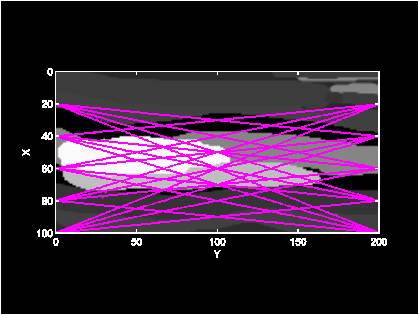
\includegraphics[width=\iwidth]{figures/tomo.jpg}
%			&
%			\includegraphics[width=\iwidth]{fig3/hydraCond-reference}
%			\\
%			\hline
		%\end{tabular}
	\end{center}
	\caption{{\it Visualizations of hydraulic conductivity with tomography sources on the left and receivers on the right. The ray paths $\Gamma_{j,k}$ are shown in pink.
	%For clarity, the flow field are shown only on a subset of the pixels. 
	}}
	\label{fig:conductivityModels}
\end{figure}
Discretizing on a staggered 2D grid using a finite volume scheme 
places $s$ and ${\bf d}$ at the cell centers. Therefore the discrete tomography experiment at each time step is then given by 
$
 	\bF{\bfs_k} = \bfd_k, \text{ for } k=1,\ldots,n.
$
The tomography experiment was setup with 20 sources in the east borehole and 20 receivers in the west borehole. The boreholes are 200m apart and 50m deep, as shown in figure....\alert{better describe the experimental setup}
 
 
\subsubsection{Comparing solution methods} % (fold)
To compare solutions methods, an experiment was conducted where data were collected from all source receiver combinations. Initial estimates of $\Sigh_0$ and the best Tikhonov regularization parameter $\alpha_0$ were obtained by a standard cooling algorithm and Pareto curve . 


\subsubsection{Mesh refinement}
compare for identical (small) time step, the designs. would be nice to get the same design results! Try to estimate the sensitivity of the design to the mesh size. how to compare? what metric?


\subsubsection{Time step restriction}
talk about the singularity of $\bT$ for time steps greater than h. What to do about this...

\subsection{DC Resistivity}



\subsubsection{Comparing solution methods} % (fold)
The big difference is whether or not we have sigma...pcg is slow

\subsubsection{Mesh refinement}
mesh refinement. If designs can be done on a coarse mesh, then it's fine to form sigma inverse. This is powerful

\subsubsection{Time step restriction}
hopefully can figure out what to do here.




\section{Numerical example 2: Iterative design, estimating the velocity as well} 



\section{Concluding Remarks}






\bibliographystyle{plain}
\bibliography{../../../../Bibliographys/ProposalBib}



\end{document}